% =====================================================================
% VERSION ENSAE, REDUCTION SFE (phase 3, 1er octobre 2026) : chapitre 9, resultats.
% Copie a texte constant de chapitres/12_resultats.tex.
% Ne changent que les titres et les renvois repares, listes dans
% reduction/phase3.md.
% Lu par main_ensae.tex seul : ne jamais le faire lire par main_institut.tex,
% qui garde chapitres/.
% =====================================================================

\chapter{Résultats}
\label{chap:resultats}
\label{part:resultats}

Les capitaux valent pour le périmètre financier étudié, non pour un assureur, et pour le
risque opérationnel d'origine informatique, sur deux périmètres de sévérité :
OpRisk, à queue lourde ($\hat\xi=0{,}595$), et PRC, plafonnée à $40$~M\euro{} par sévérité élémentaire ($\hat\xi=1{,}03$).
La variance de la sévérité étant infinie, nous donnons aussi la médiane et l'intervalle à $90\,\%$ du
bootstrap. Le niveau varie d'un facteur $41$ selon la loi de sévérité
et la fréquence (chapitre~\ref{chap:partielle}). Les rapports au socle (borne haute, largeur de bande)
varient d'au plus $33\,\%$ de leur valeur moyenne, et les deux piliers les plus coûteux restent P1 et
P4. Nous interprétons donc les écarts, non les niveaux.

À trois canaux (lecture~C), l'état conforme vaut $5\,932$~M\euro{} et à quatre canaux $6\,049$, soit
plus que le socle sans contagion du chapitre~\ref{chap:partielle}, $5\,275$~M\euro, parce qu'il
conserve une contagion.
% SOURCES-SCRIPTS: 65 66 12 16 63

\section{SCR par état de conformité}

Le besoin de capital croît de façon monotone de l'état conforme à l'état non conforme. Le
tableau~\ref{tab:scretat} donne trois lectures emboîtées : la lecture~A ne retient que la
fréquence, la lecture~B ajoute la propagation de la cascade, la lecture~C le canal de détection.

\begin{table}[htbp]\centering\small
\renewcommand{\arraystretch}{1.25}
\begin{tabular}{@{}l ccc c ccc@{}}
\toprule
& \multicolumn{3}{c}{\textbf{OpRisk} (M\euro)} & & \multicolumn{3}{c}{\textbf{PRC} (M\euro)} \\
\cmidrule(lr){2-4}\cmidrule(lr){6-8}
État & A & B & C & & A & B & C \\
\midrule
Conforme               & 8301  & 6664  & 5932  & & 2589 & 1903 & 1642 \\
Partiellement conforme & 11059 & 9625  & 9625  & & 3653 & 3118 & 3118 \\
Non conforme           & 15074 & 15074 & 16595 & & 5520 & 5520 & 6577 \\
\bottomrule
\end{tabular}
\caption{SCR par état, trois lectures (A~: fréquence ; B~: $+$~propagation ; C~:
$+$~détection). Le canal détection ne joue qu'aux extrêmes (il
% SOURCES-SCRIPTS: 16
abaisse l'état conforme et relève le non conforme), l'état partiel n'étant pas modulé.}
\label{tab:scretat}
\end{table}

\subsection*{Lectures emboîtées de l'écart}
\label{sec:chiffre-de-tete}

Quatre protocoles chiffrent l'écart entre l'état conforme et l'état non conforme, et ne diffèrent
que par le nombre de canaux qu'ils relâchent.

\begin{center}\footnotesize
\renewcommand{\arraystretch}{1.25}
\begin{tabular}{@{}l c r r r@{}}
\toprule
\textbf{Lecture} & \textbf{canaux} & \textbf{conforme} & \textbf{non conf.} & \textbf{facteur} \\
\midrule
Score de conformité seul, $g$ figé au niveau NC & 1 & 7987 & 16\,847 & $2{,}11$ \\
Fréquence $+$ propagation (lecture~B) & 2 & 6664 & 15\,074 & $2{,}26$ \\
$+$ détection (lecture~C) & 3 & 5932 & 16\,595 & $2{,}80$ \\
\textbf{$+$ accumulation P4 (les quatre canaux)} & \textbf{4} & \textbf{6049} & \textbf{20\,188}
& $\mathbf{3{,}34}$ \\
\bottomrule
\end{tabular}
\end{center}

\vspace{4pt}
\noindent La lecture à quatre canaux donne $6\,049 \to 20\,188$~M\euro{} sur le périmètre financier étudié (sévérité OpRisk).
Le facteur est de $3{,}34$ et l'écart de $14\,139$~M\euro{}, d'écart-type $734$~M\euro{} entre quatre graines
(erreur type de la moyenne : $367$~M\euro{}). Elle seule définit l'état conforme sur tous les canaux.
Les autres lectures sont des remédiations partielles : la première conserve la propagation non conforme ; les deux suivantes, la détection ou l'accumulation non conforme.
La première ligne fixe $g$ au niveau NC et diffère de la lecture~A précédente.

Nous
incluons le canal de détection parce que son effet est résolu, avec $2\,928 \pm 343$~M\euro{} en
valeur de Shapley, $4\,562 \pm 819$ en marginal de fermeture (figure~\ref{fig:canaux-rapport}) et
un signe constant sur seize graines. Le facteur entre états repose sur des hypothèses de conformité.
Il ne mesure pas un effet observé de DORA, les états de conformité des entités n'étant pas publiés.

\begin{figure}[H]\centering
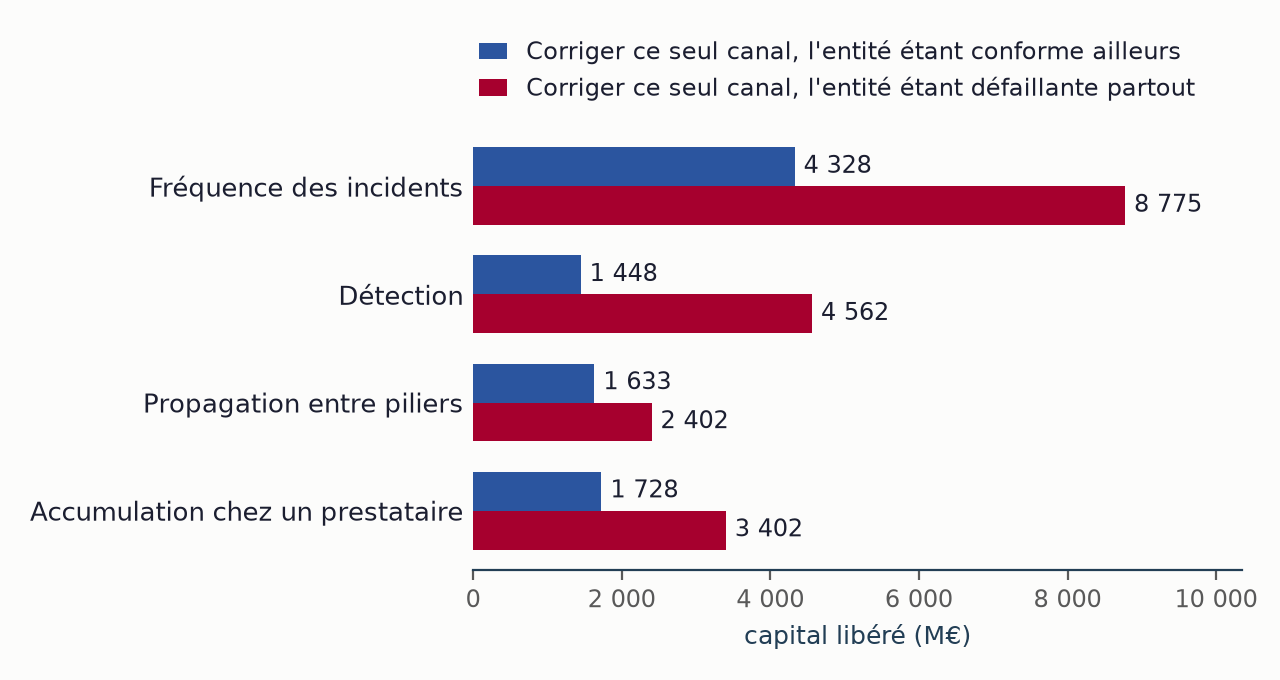
\includegraphics[width=0.72\textwidth]{N1_canaux_note.png}
\caption{Capital libéré par la correction d'un seul canal, selon que l'entité est déjà conforme sur
les trois autres canaux (effet isolé) ou défaillante partout (effet de fermeture), en M\euro{} à
l'échelle du secteur.}
% SOURCES-SCRIPTS: 101 68
\label{fig:canaux-rapport}
\end{figure}

Le facteur se compare d'une lecture à l'autre, non l'écart en euros. Entre les
deux premières lignes, l'écart passe de $8\,860$ à $8\,410$~M\euro{} alors que le facteur monte, la
base conforme passant de $7\,987$ à $6\,664$~M\euro. Les canaux se multiplient presque, le produit
des quatre facteurs isolés étant de $3{,}47$ pour un facteur publié de $3{,}34$
(figure~\ref{fig:treillis-canaux-rapport}). Les quatre effets isolés somment à $9\,138$~M\euro{} et
l'écart de $14\,139$ les dépasse de $5\,001$, l'interaction. Elle correspond à ce que donnerait un
produit des facteurs ($5\,813$~M\euro{} pour un modèle purement multiplicatif) plus qu'à un effet
propre de la cascade (\S\ref{sec:inverse}). Les
trajectoires et la priorisation restent conduites en lecture~B, car elles concernent l'ordre de
remédiation, que le canal ajouté ne déplace pas.

\begin{figure}[H]\centering
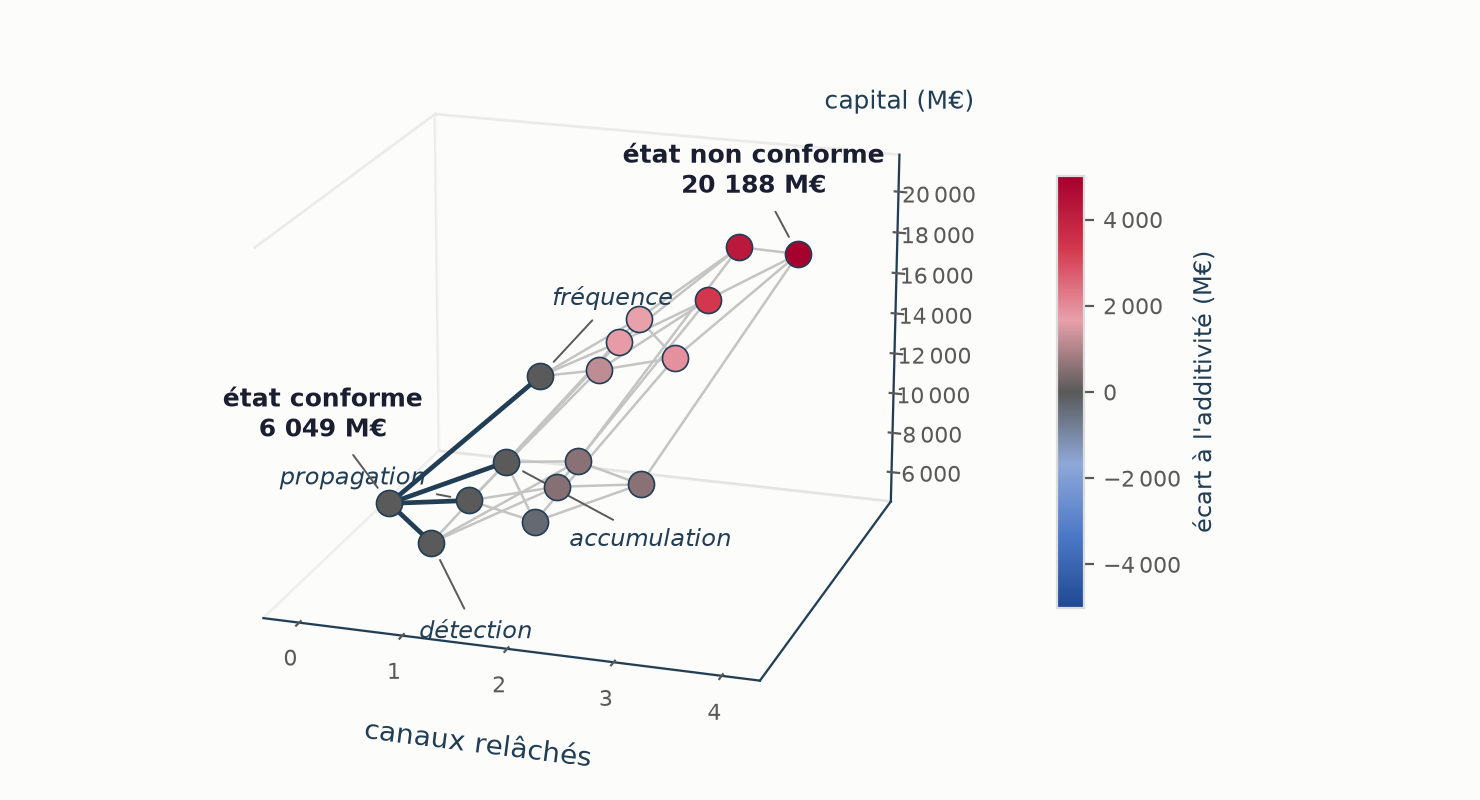
\includegraphics[width=0.95\textwidth]{treillis_canaux.png}
\caption{Les seize configurations des quatre canaux, rangées par nombre de canaux relâchés. La
hauteur est le capital ; les deux extrémités sont les états publiés, $6\,049$ et
$20\,188$~M\euro{}, et tout sommet intermédiaire est une remédiation partielle. Chaque arête monte.
La couleur est l'écart à l'additivité, capital observé moins la somme des quatre effets isolés :
$+5\,001$~M\euro{} au sommet complet, $-330$ sur la seule paire négative, propagation et
accumulation. Le troisième axe sépare les configurations de même rang et ne porte aucune grandeur.}
% SOURCES-SCRIPTS: 68 108
\label{fig:treillis-canaux-rapport}
\end{figure}

Nous obtenons le surcoût $\Delta_{\text{DORA}}=\mathrm{SCR}(\text{NC})-\mathrm{SCR}(\text{C})$, à
graine Monte-Carlo commune, par bootstrap à deux niveaux (multiplicateurs et sévérité), et
$100\,\%$ des tirages sont positifs (tableau~\ref{tab:delta}).

\begin{table}[htbp]\centering\small
\renewcommand{\arraystretch}{1.25}
\begin{tabular}{@{}l cc@{}}
\toprule
& médiane & IC90\,\% \\
\midrule
$\Delta_{\text{DORA}}$ NC vs C (OpRisk) & 7401 & $[2830\,;38793]$ \\
$\Delta_{\text{DORA}}$ PC vs C (OpRisk) & 2556 & $[963\,;12768]$  \\
$\Delta_{\text{DORA}}$ NC vs C (PRC)    & 3668 & $[3201\,;4094]$  \\
$\Delta_{\text{DORA}}$ PC vs C (PRC)    & 1257 & $[1077\,;1466]$  \\
\bottomrule
\end{tabular}
\caption{Surcoût de non-conformité (M\euro), lecture B, bootstrap deux niveaux. Côté OpRisk la
sévérité de queue est ré-échantillonnée sur les $91$ excès réels ; l'intervalle reste large parce
que la queue l'est.}
\label{tab:delta}
\end{table}

La queue d'indice $0{,}60$ explique la largeur de l'intervalle OpRisk ; le surcoût reste positif dans tous les tirages.
Cet intervalle concerne la lecture B. Pour les quatre canaux, seule la dispersion entre graines est donnée (écart-type de $734$~M\euro), sans l'incertitude d'estimation de la queue.
Réinjecter le résidu de conversion de \citet{jacobs2014}, $0{,}523$ en logarithme (facteur $2{,}4$ à $90\,\%$),
laisse l'intervalle PRC étroit et déplace le surcoût de $7\,\%$.

% SOURCES-SCRIPTS: 25 16 43 67 68 100 14 21 74

\section{Décomposition par pilier}

Si l'on bascule un pilier à la fois de conforme à non conforme, le surcoût se décompose selon le
classement $P1>P4>P2>P3>P5$, celui du classement ROOT du modèle qualitatif. Cet accord est attendu et
ne constitue pas une validation indépendante, car les amorces de la cascade sont semées selon ROOT, posé par le même expert que
la matrice dont $W$ est tirée (\S\ref{sec:baremes}).

Les surcoûts isolés ne somment pas au surcoût total, la différence étant une interaction qu'un modèle sans
propagation ne produit pas. Sur la VaR à $99{,}5\,\%$ OpRisk, son signe n'est pas résolu, de $-137$ à
$+1\,395$~M\euro{} sur six graines de $60\,000$ années, positive quatre fois sur six. Elle est
positive sur les six graines en perte moyenne, de $+532$ à $+659$~M\euro{} côté OpRisk et $+827$
côté PRC, et dans la VaR du périmètre PRC, dont le plafond tronque la queue ($+905$~M\euro).

L'attribution par pilier exige donc une règle additive, la valeur de Shapley. Cette
interaction entre piliers ne s'additionne pas à l'interaction de $+5\,001$~M\euro{} entre les quatre
canaux, de signe résolu (\S\ref{sec:kpi}) : elles décomposent l'écart selon deux axes, les piliers et
les canaux, et l'attribution par pilier se lit sur le protocole du tableau~\ref{tab:shapley}.
% SOURCES-SCRIPTS: 16b 20b 68

\section{Allocation du capital par Shapley et Euler}
\label{sec:allocation}

La valeur de Shapley attribue le surcoût aux piliers sources de la non-conformité, interaction
comprise, et indique ainsi qui le supporte. La règle d'Euler, appliquée à la moyenne de queue
de $L$, indique sur quels piliers touchés se loge la perte au-delà du quantile.
% SOURCES-SCRIPTS: 20

\subsection{Attribution par Shapley}

On munit les piliers d'une fonction caractéristique
\[
v(S) \;=\; \mathrm{SCR}\bigl(S \text{ en NC},\ \text{reste C}\bigr)-\mathrm{SCR}(\text{tous C}),
\qquad S \subseteq \{P1,\dots,P5\},
\]
calculée par la cascade sur les $2^5$ configurations à graine Monte-Carlo commune. La valeur de
Shapley
\[
\varphi_j \;=\; \sum_{S \subseteq \{P1,\dots,P5\}\setminus\{j\}}
\frac{|S|!\,\bigl(5-|S|-1\bigr)!}{5!}\,\bigl[v(S\cup\{j\})-v(S)\bigr]
\]
moyenne la contribution de $j$ sur tous les ordres d'arrivée, et
$\sum_j \varphi_j = v(\text{tous}) = \Delta_{\text{DORA}}$ \citep{Shapley1953}. Son
emploi en allocation de capital remonte à \citet{denault2001}, et son usage actuariel sous
Solvabilité~II est documenté \citep{Decupere2011}. Avec cinq piliers, on énumère les $5!$
ordres, sans les algorithmes par échantillonnage \citep{CastroGomezTejada2009, SongNelsonStaum2016}.
Le tableau~\ref{tab:shapley} en donne les valeurs.

\begin{table}[H]\centering\small
\renewcommand{\arraystretch}{1.25}
\begin{tabular}{@{}l rrr c rrr@{}}
\toprule
& \multicolumn{3}{c}{OpRisk} & & \multicolumn{3}{c}{PRC} \\
\cmidrule{2-4}\cmidrule{6-8}
pilier & marginal & $\varphi_j$ & part & & marginal & $\varphi_j$ & part \\
\midrule
P1 gouvernance & 3481 & 3717 & $34{,}0\,\%$ & & 1375 & 1608 & $32{,}4\,\%$ \\
P4 tiers       & 2658 & 2810 & $25{,}7\,\%$ & & 1075 & 1252 & $25{,}3\,\%$ \\
P2 incidents   & 1634 & 1867 & $17{,}1\,\%$ & &  721 &  920 & $18{,}6\,\%$ \\
P3 tests       & 1094 & 1484 & $13{,}6\,\%$ & &  571 &  738 & $14{,}9\,\%$ \\
P5 partage     &  665 & 1048 &  $9{,}6\,\%$ & &  311 &  438 &  $8{,}8\,\%$ \\
\midrule
somme          & 9531 & 10\,927 & $100{,}0\,\%$ & & 4052 & 4957 & $100{,}0\,\%$ \\
\bottomrule
\end{tabular}
\caption{Valeur de Shapley du surcoût $\Delta_{\text{DORA}}$ (M\euro, périmètre financier étudié, trois canaux : fréquence, propagation, détection ; base
conforme $6\,085$ du moteur par pilier, qui s'écarte de quelques pour cent de la lecture~C du tableau~\ref{tab:scretat}).}
% SOURCES-SCRIPTS: 16b
\label{tab:shapley}
\end{table}

Le classement de Shapley reproduit le classement ROOT sur les deux périmètres, en partie
mécaniquement, les amorces étant semées selon ROOT (parts $30/27/18/15/9\,\%$). La part de P1,
$34\,\%$, excède toutefois sa part d'amorce de $30\,\%$, ce qui traduit l'effet propre de la
propagation, P1 étant l'émetteur le plus fort de $W$.
% SOURCES-SCRIPTS: 20

\subsection{Allocation par Euler}

La règle d'Euler \citep{tasche1999} calcule
$C_j = \mathbb{E}\bigl[L_j \mid L \ge \VaR_{99{,}5\,\%}\bigr]$, où $L_j$ est la perte du pilier touché
$j$. Ces contributions somment à $\TVaR_{99{,}5\,\%}(L)$ et non au quantile : c'est une allocation de
la moyenne de queue, lue comme diagnostic de la localisation du capital. Côté PRC, l'allocation est stable et presque plate (P2 $23\,\%$, P4 $23\,\%$, P1 $20\,\%$, P3
$18\,\%$, P5 $17\,\%$), le plafond de sévérité tronquant la queue ($\TVaR = 6\,795 \approx \VaR =
6\,573$~M\euro). Côté OpRisk, les parts moyennes sont stables, mais l'allocation de la queue
extrême ne l'est pas. En effet, avec $\xi \approx 0{,}6 > 0{,}5$, la sévérité est de variance infinie
et le classement conditionnel bascule d'une résolution de simulation à l'autre. Nous retenons donc
l'allocation du périmètre PRC.
% SOURCES-SCRIPTS: 16b

Le besoin de capital publié est partout le quantile $\VaR_{99{,}5\,\%}(L)$ non centré, la perte
attendue d'une non-conformité n'étant pas couverte par une provision. Aucune grandeur de couverture
n'est une TVaR. La mesure de queue ne sert qu'au diagnostic, à deux titres. Elle sert d'abord de
base à l'allocation d'Euler, qui répartit la TVaR et non le quantile. Elle indique aussi la forme de la queue, le rapport
$\TVaR_{99{,}5\,\%}(L)/\VaR_{99{,}5\,\%}(L) \approx 2{,}1$ se comparant à son asymptote
$1/(1-\xi) = 2{,}5$. Ce rapport est de $2{,}10$ à l'état tous non conforme et de $2{,}17$ sur la
calibration de référence. Sous la calibration PRC non plafonnée, $\hat\xi=1{,}033>1$ rend l'espérance infinie, de
sorte que la mesure de queue n'existe pas et ne peut fonder un besoin de capital ; l'allocation du
périmètre PRC porte sur la sévérité plafonnée, dont les moments sont finis.
% SOURCES-SCRIPTS: 20 67 73

\section{Trajectoire du capital}
\label{sec:res-traj}

Le long de la mise en conformité, partant d'une répartition supposée des états (NC~$35\,\%$, PC~$35\,\%$,
C~$30\,\%$), en lecture~B, le capital OpRisk passe de $10\,752$ à $7\,041$~M\euro{} en cinq ans, vers le SCR
conforme. Le surcoût résiduel tend vers zéro, et son intégrale, à un coût de capital près, est le
coût de portage de la non-conformité pendant la remédiation. La bande à $90\,\%$ reste haute en
environnement dégradé, scénario où le capital importe le plus.
% SOURCES-SCRIPTS: 17

\section{Priorisation de la remédiation}
\label{sec:res-prio}

Sous budget contraint, un pilier remédié à la fois, nous énumérons les $120$ ordres, dont
l'optimal, $P1\to P4\to P2\to P3\to P5$, est égal à l'ordre ROOT et distinct de l'ordre glouton par
valeur d'accélération. L'écart de capital intégré entre le pire ordre et l'optimal atteint
$21\,\%$. Remédier au coup par coup le pilier au plus fort gain immédiat coûte plus cher, car les
interactions de cascade imposent de raisonner sur l'horizon entier.
% SOURCES-SCRIPTS: 18

Le test de résistance inverse fixe le capital et cherche les états qui le produisent, la monotonie
du \S\ref{sec:kpi} rendant croissant l'ensemble des configurations atteignant une cible, donc décrit
par ses éléments minimaux. Le canal de fréquence seul atteint $10\,377$~M\euro, soit $1{,}72$ fois
l'état conforme, et les trois autres canaux réunis n'atteignent que $11\,413$ ($1{,}89$ fois).
Toute cible sous le premier seuil se produit par un canal unique, et toute cible au-dessus du second
exige la fréquence. Aucun autre canal seul n'atteint $8\,000$~M\euro{} (\S\ref{sec:inverse}).
% SOURCES-SCRIPTS: 92

\section{Robustesse}
\label{sec:res-robustesse}

Le niveau du capital varie beaucoup avec les leviers testés, l'indice de queue dominant avec
un facteur de l'ordre de $6$. Le signe du surcoût et la priorité de P1 tiennent pourtant sur tous
ces leviers. L'ordre de remédiation optimal ne dépend que des SCR par configuration, et il
est donc invariant aux taux de transition de la chaîne de Markov, qui ne fixent que le calendrier.
% SOURCES-SCRIPTS: 19

Nous menons ces tests à matrice $W$ fixée. Sur l'ensemble admissible (chapitre~\ref{chap:partielle}),
P1 et P4 sont presque à égalité, P1 arrivant premier dans $43{,}6\,\%$ des configurations et P4 dans
$37{,}7\,\%$, avec un écart de regret maximal de $1{,}5\,\%$. P1 et P4 devancent P2, P3 et
P5, et P5 n'arrive jamais en tête. Les rapports post-incident sur-attribuant à la gouvernance, nous
dégradons l'émission de P1 par $W_{1k}\to(1-a)W_{1k}$, et le classement tient jusqu'à $a=0{,}25$
puis bascule vers P4 à $a=0{,}50$. Même à $a=1$, le niveau ne perd que $24{,}8\,\%$, l'équivalent de
$0{,}81$ fois la largeur de la bande d'identification.
% SOURCES-SCRIPTS: 30 64 22 67

\section{Sensibilité aux probabilités de propagation}
\label{sec:sensibilite-propagation}
% SOURCES-SCRIPTS: 15 76 30 66 68

Le niveau de la propagation est un facteur d'échelle posé, qui se stresse, tandis que sa direction
n'est pas identifiable et se borne. Mesurée en élasticités, à perturbation relative de $10\,\%$ d'un paramètre
à la fois, la sensibilité classe les leviers comme suit.

\begin{center}\footnotesize
\renewcommand{\arraystretch}{1.15}
\begin{tabular}{@{}l l r@{}}
\toprule
\textbf{Levier} & \textbf{Statut} & \textbf{Élasticité} \\
\midrule
Indice de queue $\xi$ & estimé & $3{,}79$ \\
Échelle $\sigma$ & estimé & $0{,}97$ \\
Taux de dépassement $p_u$ & estimé & $0{,}82$ \\
Fréquence $\lambda$ & estimé & $0{,}45$ \\
Sur-dispersion $\varphi$ & posé & $-0{,}44$ \\
\textbf{Gain de propagation} $\boldsymbol{g}$ & \textbf{posé} & $\mathbf{0{,}37}$ \\
Seuil $u$ seul & choix de méthode & $0{,}03$ \\
\bottomrule
\end{tabular}
\end{center}

\vspace{4pt}
\noindent La propagation a l'élasticité la plus faible des leviers substantiels, $0{,}37$ contre
$3{,}79$ pour l'indice de queue. Le même classement ressort de l'ablation, qui fait tomber la VaR de
$20\,\%$ en retirant la propagation et de $76\,\%$ en retirant la queue lourde. La thèse ne dépend pas des trois valeurs
posées de $g$, le capital étant croissant en $g$ (\S\ref{sec:invariance-g}). Nous bornons la direction.
À ignorance totale, la largeur de l'ensemble admissible s'élève à $1\,839$~M\euro, soit $34{,}9\,\%$
du socle, et elle croît avec le degré d'ignorance ($336$, $695$, $1\,083$ puis $1\,839$~M\euro{} pour
degrés d'ignorance de $0{,}25$, $0{,}50$, $0{,}75$ et $1$). Le déplacement
conjoint du seuil et des paramètres de queue réajustés ($\xi$, $\sigma$, $p_u$) fait passer le
surcoût de $4\,862$ à $12\,944$~M\euro, sur la base propre du tornado, distincte du chiffre de tête.
Le seuil seul pèse peu ($0{,}03$), et l'incertitude numérique tient d'abord à l'ajustement de la queue.
% SOURCES-SCRIPTS: 81

\section{Comparaison de modèles de dépendance}
\label{sec:benchmark}

Comme la cascade remplace l'agrégation par copule d'un modèle LDA, nous la confrontons à des modèles à copule
de mêmes marges par pilier, à graines communes, sur le périmètre OpRisk. À corrélation
calée, la copule gaussienne retombe sur le SCR de la cascade ($+0{,}1\,\%$ sur une graine,
$+4{,}8\,\%$ en moyenne sur quatre, sous son propre bruit). En queue lourde, le quantile annuel
tient à la perte unique dominante, et le niveau n'identifie pas la dépendance. La Student
($\nu = 4$) le surestime de $17\,\%$ en forçant des co-extrêmes que la cascade ne produit pas
($2{,}28$ piliers extrêmes par année de queue contre $1{,}12$). Le préprint de cascade climatique
\citep{ccrn2026} emploie le même protocole.

Basculer un pilier en non-conformité est cependant une intervention. Le modèle à copule y donne un
surcoût inférieur de $38\,\%$, $6\,760$~M\euro{} contre $10\,927$ pour la cascade, la copule n'ayant
pas de mécanisme de propagation. Son interaction moyenne est nulle par construction, tandis que la
cascade en produit $+560$~M\euro{}. La priorité qu'il implique s'inverse sur P2 et P3. Sa dépendance
ne durcit pas non plus lorsque la conformité se dégrade, alors que c'est le canal de propagation que la non-conformité
déplace ($g$ de $0{,}45$ à $0{,}90$).
% SOURCES-SCRIPTS: 23 80 67

\section{Comparaison avec les cadres réglementaires}
\label{sec:regard-reglementaire}

Sur le même écart de capital entre profil conforme et profil non conforme, trois cadres expriment des
fractions différentes de l'effet de la conformité (tableau~\ref{tab:benchmark-sf}).

\begin{table}[H]\centering\small
\renewcommand{\arraystretch}{1.25}
\begin{tabular}{@{}l r r@{}}
\toprule
\textbf{Cadre} & \textbf{$\Delta$ capital C$\to$NC} & \textbf{part de l'effet cascade} \\
\midrule
Formule Standard (Solvabilité~II) & $0$~M\euro{} & $0\,\%$ \\
LDA-copule (dépendance symétrique) & $6\,760$~M\euro{} & $62\,\%$ \\
Cascade dirigée & $10\,927$~M\euro{} & $100\,\%$ (référence) \\
\bottomrule
\end{tabular}
\caption{Fraction de l'effet DORA que chaque cadre sait exprimer (périmètre financier étudié, trois
canaux, accumulation exclue, protocole du tableau~\ref{tab:shapley}).}
\label{tab:benchmark-sf}
\end{table}

La charge de risque opérationnel de l'équation~\eqref{reg:eq:scrop} ne dépend que du volume. Elle
est identique pour une entité exemplaire et pour une entité défaillante sur DORA. La copule capte
$62\,\%$ de l'effet, par les canaux fréquence et détection, mais manque la propagation.
% SOURCES-SCRIPTS: 27 67

\section{Descente à l'échelle d'une entité}
\label{sec:ancrage}

Pour l'entité notionnelle, le repère forfaitaire de la Formule Standard est d'environ
$450$~M\euro. Le socle sans contagion du périmètre financier étudié vaut $5\,275$~M\euro{} ;
les deux ne se comparent pas. Au niveau du
sinistre unique, le quantile de sévérité ($663$~M\euro) et sa moyenne de queue ($1\,752$~M\euro)
sont en revanche du même ordre que les grandes pertes cyber observées ($1\,288$ à $2\,208$~M\euro). À matrice $W$ et moteur inchangés, une entité d'actifs $A$ reçoit une fréquence et une
sévérité lues à sa taille :
\begin{equation}\label{eq:descente}
\begin{gathered}
\lambda(A)=\lambda_c\Big(\frac{A}{A_c}\Big)^{b_\lambda},\qquad
m(A)=\Big(\frac{A}{A_m}\Big)^{b},\\
X=m(A)\sum_{k\in S_a}Y_k,\qquad
\mathcal{B}(A)=\VaR_{99{,}5\,\%}\Big(\sum_{n=1}^{N}X_n\Big),
\end{gathered}
\end{equation}
où $N$ suit la binomiale négative de moyenne $\lambda(A)$ et de surdispersion $\varphi$, $S_a$ est
l'ensemble des piliers touchés depuis l'amorce $a$ et les $Y_k$ les sévérités GPD calibrées. Nous
estimons les élasticités à $b_\lambda = 0{,}074$ et $b = 0{,}087$, d'où $m = 0{,}854$ à la taille
de l'entité notionnelle.

\begin{table}[htbp]\centering
\small
\begin{tabular}{lrrrr}
\toprule
Lecture & $\lambda$ (an$^{-1}$) & sévérité & SCR $99{,}5\,\%$ & Perte moyenne \\
\midrule
Secteur financier mondial & $21{,}56$ & $\times 1$ & $8\,123$~M\euro & $983$~M\euro \\
Seuil \og{}$\geq 10$ événements\fg{} & $0{,}210$ & $\times 1$ & $488$~M\euro & $9{,}7$~M\euro \\
Seuil \og{}toutes firmes\fg{} & $0{,}100$ & $\times 1$ & $229$~M\euro & $4{,}6$~M\euro \\
$\lambda$ lu à la taille de la cible & $0{,}092$ & $\times 1$ & $198$~M\euro & $4{,}3$~M\euro \\
\textbf{Les deux canaux composés} & $\mathbf{0{,}092}$ & $\mathbf{\times 0{,}854}$ &
$\mathbf{169}$~M\euro & $\mathbf{3{,}6}$~M\euro \\
\bottomrule
\end{tabular}
\caption{Le même modèle lu à plusieurs échelles ; seules la fréquence d'amorce et l'échelle de
sévérité changent. La dernière ligne prend fréquence et sévérité à la taille de l'entité notionnelle.}
\label{tab:echelle}
\end{table}

Diviser $\lambda$ par $235$ divise la perte moyenne par $270$ mais le capital par $48$ seulement, car
le quantile extrême dépend du plus grand sinistre. Le chiffre d'entité est une bande,
$[131{,}5\,;183{,}3]$~M\euro{} sur les $1\,024$ sommets admissibles, qui ne traduit que l'ignorance de
la direction, et les $169$~M\euro{} restent une extrapolation d'ordre de grandeur
(\S\ref{sec:entites-reelles}). À cette échelle, la bande
d'identification mesure $51{,}7$~M\euro. L'indice de queue, parcouru sur son intervalle à $90\,\%$
($\xi \in [0{,}304\,;0{,}831]$), fait varier le
besoin de capital de l'entité de $51{,}5$~M\euro, de $140{,}9$ à $191{,}6$~M\euro.

Le gain de propagation pris à ses trois valeurs d'état ($0{,}45$, $0{,}68$, $0{,}90$) fait passer le
besoin de capital de l'entité de $116$ à $143$ puis $169$~M\euro, soit $+45\,\%$ par le seul canal de contagion
(figure~\ref{fig:invariance-g-rapport}). Le repère forfaitaire reste à $450$~M\euro. Ce scénario d'écartement repose sur une correspondance
posée entre état et $g$. Les correspondances testées entre état et $g$ conservent le signe de l'écart (\S\ref{sec:invariance-g}) ; cette vérification sur grille ne démontre pas la monotonie générale du moteur de marche.
% SOURCES-SCRIPTS: 60 49

\begin{figure}[H]\centering
\figover{S23_invariance_conformite.png}
\caption{Capital d'entité et valeurs du gain de propagation $g$. (a)~Le capital croît avec $g$, sur
vingt points de grille à nombres aléatoires communs, quand la charge forfaitaire ne dépend pas de
l'état. (b)~Cinq correspondances entre état et $g$, de très étroite à large : toutes respectent
l'ordre du capital, et le forfait reste plat. (c)~L'amplitude de l'écart ne dépend que de
l'écartement $g_{NC}-g_C$ ; la valeur retenue est marquée, et elle seule relève du scénario.}
% SOURCES-SCRIPTS: 66 67
\label{fig:invariance-g-rapport}
\end{figure}

\section{Application à quatre entités}
\label{sec:entites-reelles}

L'entité notionnelle est posée à $20\,000$~M\$ d'actifs et $15\,000$~M\euro{} de provisions. Nous
appliquons la méthode à quatre assureurs à partir de leurs rapports SFCR de l'exercice 2024, qui
donnent provisions techniques, fonds propres éligibles et SCR. Le besoin de chaque entité est
$\mathcal{B}(A)$ de l'équation~\eqref{eq:descente}, en point au gain de propagation non conforme et
en bande sur les sommets admissibles. Aucun module DORA n'existant en Formule Standard, ce besoin
relève de l'ORSA (section~\ref{chap:reglementaire}), et son rapport au SCR publié est une mise à
l'échelle, pas une part. Nous désignons les entités par leur classe, car le modèle n'utilise que leur
bilan, leur état de conformité étant supposé.

\begin{center}\small
\renewcommand{\arraystretch}{1.25}
\begin{tabular}{@{}l r r r r r@{}}
\toprule
\textbf{Entité} & \textbf{Actifs} & \textbf{SCR publié} & \textbf{Besoin ORSA} &
\textbf{Bande} & \textbf{Rapport} \\
 & M\euro & M\euro & M\euro & M\euro & \\
\midrule
Assureur non-vie A & $2\,319$ & $425$ & $112$ & $[88\,;122]$ & $26{,}4\,\%$ \\
Assureur non-vie B & $5\,305$ & $812$ & $136$ & $[104\,;146]$ & $16{,}7\,\%$ \\
Assureur vie C & $37\,845$ & $1\,587$ & $196$ & $[149\,;213]$ & $12{,}3\,\%$ \\
\textbf{Assureur vie D} & $\mathbf{309\,800}$ & $\mathbf{14\,800}$ & $\mathbf{294}$ &
$\mathbf{[233\,;316]}$ & $\mathbf{2{,}0\,\%}$ \\
\midrule
\emph{Entité notionnelle} & $19\,231$ & -- & $169$ & $[132\,;183]$ & -- \\
\bottomrule
\end{tabular}
\end{center}

\vspace{2pt}
\noindent Les quatre SCR sont publiés, les deux assureurs non-vie les donnant dans leur état
S.25.01, à $425$ et $812{,}5$~M\euro. Seul le total d'actif de trois entités est déduit, par
l'identité comptable, et l'approximation est conservatrice. Les mêmes états publient également le
module de risque opérationnel. Le repère de $3\,\%$ des provisions donne $54{,}1$ contre $59$ publié
sur la première entité non-vie, et $62{,}1$ contre $39{,}7$ sur la seconde, soit $-8\,\%$ et $+56\,\%$. Ce
repère n'est donc qu'un ordre de grandeur, jamais une borne.

Sur la plus grande entité, $310$~Md\euro{} d'actifs, le besoin représente $2{,}0\,\%$ de son SCR
publié, avec $294$~M\euro{} en point et $[233\,;316]$ en bande. L'écart entre états de conformité
subsiste à toutes les tailles, de $+41\,\%$ à $+49\,\%$. La charge décroît toutefois bien moins vite
que la taille, puisqu'un facteur $134$ sur les actifs ne divise la sévérité que par $1{,}53$ et la
fréquence que par $1{,}44$. Le rapport passe ainsi de $2{,}0\,\%$ à $26{,}4\,\%$.

Un critère de $10\,\%$ du SCR total pour un seul risque de non-conformité, posé et non mesuré, place
la bascule entre $37\,845$ et $309\,800$~M\euro{} d'actifs. Le levier propre des entités, de
$4{,}2$ à $18{,}3\,\%$, module aussi cet ordre de grandeur. L'élasticité corrige l'échelle de la
sévérité, mais sa forme reste celle de grandes institutions financières. L'entité notionnelle, à
$19\,231$~M\euro{} d'actifs, se situe sous cette bascule, dans une zone où la mise à l'échelle reste incertaine. Les $169$~M\euro{} sont donc une extrapolation, dont rien ne garantit qu'elle majore le besoin réel ; le critère de poids dans le SCR ne fixe pas de domaine de validité statistique. Au levier médian des quatre entités ($10{,}0\,\%$), qui donne
$1\,932$~M\euro{} de SCR, la charge en représenterait $9\,\%$, sous le critère. L'argument de taille justifie une réserve d'extrapolation, sans prouver que le chiffre surestime le risque réel.

La thèse concerne l'écart entre états, un rapport, qui survit à une erreur de niveau commune aux
trois états. Comme les entités ne publient pas leur état de conformité, nous mesurons une exposition
sous un état supposé, jamais une non-conformité constatée.
% SOURCES-SCRIPTS: 65

\section{Agrégation au capital total}
\label{sec:agregation-scr}

Sous Solvabilité~II, le risque opérationnel n'entre pas dans la matrice de corrélation du BSCR,
selon l'identité $\mathrm{SCR} = \mathrm{BSCR} + \mathrm{Adj} + \mathrm{SCR}_{Op}$ de la
section~\ref{chap:reglementaire}. Nous comparons deux conventions hypothétiques pour agréger un écart $D$ en ORSA : l'ajouter en entier, comme le SCR opérationnel, après en avoir retranché le risque informatique que celui-ci couvre déjà, ou le traiter comme un module corrélé à $\rho$ avec le BSCR :
\begin{equation}\label{eq:agregation}
\Delta\mathrm{SCR}_{\text{additif}} = D,\qquad
\Delta\mathrm{SCR}_{\rho}=\sqrt{\mathrm{BSCR}^2+2\rho\,\mathrm{BSCR}\,D+D^2}-\mathrm{BSCR}
=\tau(\rho,d)\,D,
\end{equation}
\begin{equation}\label{eq:tau}
\tau(\rho,d)=\frac{\sqrt{1+2\rho d+d^2}-1}{d}
=\rho+\frac{d}{2}\bigl(1-\rho^2\bigr)+O(d^2),\qquad d=\frac{D}{\mathrm{BSCR}} .
\end{equation}
Pour $D$ petit devant le BSCR, la convention corrélée en retient environ $\rho D$, la convention additive $D$. Le BSCR n'étant pas publié, nous le minorons par $\mathrm{SCR}-\mathrm{SCR}_{Op}$ si $\mathrm{Adj}\le0$, et par $\mathrm{SCR}/1{,}3$ si les frais des unités de compte sont nuls ($Exp_{ul}=0$) ; pour les assureurs vie, où ce n'est pas vérifié, les valeurs du tableau ne sont pas des majorants garantis.

\begin{center}\small
\renewcommand{\arraystretch}{1.25}
\begin{tabular}{@{}l r r r r@{}}
\toprule
\textbf{Entité} & \textbf{Écart $D$, contagion} & \textbf{$d = D/\mathrm{BSCR}$} &
\textbf{$\tau$ à $\rho = 0{,}25$} & \textbf{additif / corrélé} \\
 & M\euro & & & \\
\midrule
Assureur non-vie A & $34{,}9$ & $0{,}0954$ & $29{,}4\,\%$ & $3{,}41$ \\
Assureur non-vie B & $44{,}4$ & $0{,}0575$ & $27{,}7\,\%$ & $3{,}62$ \\
Assureur vie C & $62{,}7$ & $0{,}0514$ & $27{,}4\,\%$ & $3{,}65$ \\
Assureur vie D & $86{,}0$ & $0{,}0076$ & $25{,}4\,\%$ & $3{,}94$ \\
\bottomrule
\end{tabular}
\end{center}

\vspace{2pt}
\noindent L'écart $D$, limité à la contagion, est un plancher. À $\rho = 0{,}25$, le facteur $1/\tau$
va de $3{,}4$ à $3{,}9$ pour des tailles dans un rapport $134$, et de $2{,}6$ à $3{,}8$ en lecture de niveau.
L'écart représente $0{,}58\,\%$ à $8{,}21\,\%$ du SCR publié et est reconnu intégralement en convention additive.
Pour l'assureur non-vie~A, le besoin atteint $2{,}21$ fois le plafond de $0{,}3\,\mathrm{BSCR}$ du risque opérationnel.
À $\rho=0{,}25$ (posé), un euro d'écart compte trois à quatre fois plus en additif qu'en corrélé, sans économie reconnue par le régulateur.
% SOURCES-SCRIPTS: 95 65

\section{Détention du capital et transfert du risque}
\label{sec:detenir-transferer}
% SOURCES-SCRIPTS: 60

Le portage annuel est fixé à $\mathrm{CoC}\times\mathrm{SCR}$ : $6\,\%$, puis $4{,}75\,\%$ au 30 janvier 2027 (directive (UE)~2025/2).
Le ratio sinistres/primes de $48{,}5\,\%$ donne une prime d'environ $2{,}1$ fois la perte attendue.
Les $169$~M\euro{} de capital pour $3{,}6$~M\euro{} de perte moyenne donnent un multiple de $47$, contre $8{,}3$ sur le périmètre étudié.

Un traité annuel en excès de perte, sans rétention, cède $\min(L,\ell)$ de la charge $L$, pour une portée $\ell$.
Son coût de financement est
\begin{equation}\label{eq:cout-transfert}
C(\ell)=\frac{\E\bigl[\min(L,\ell)\bigr]}{\mathrm{LR}}
+\mathrm{CoC}\cdot\VaR_{99{,}5\,\%}\bigl(L-\min(L,\ell)\bigr),
\end{equation}
où $\mathrm{LR}$ est le ratio de sinistralité et $\mathrm{CoC}$ le taux de coût du capital. Le minimum,
en $\ell^\star=\mathrm{SCR}=169$~M\euro{}, fait passer le coût de $8{,}0$ à $2{,}9$~M\euro{} par
an, soit $-64\,\%$. Pertes conservées comprises, il passe de $11{,}67$ à $5{,}12$~M\euro{} ($-56\,\%$).
Capacité du marché, exclusions et contrepartie réduisent ce gain idéalisé.

Face au meilleur traité, détenir le risque coûte moins cher au-delà de $64\,\%$ de portée sans allègement de capital,
ou $81{,}5\,\%$ pertes conservées comprises.
Si la conformité ramène $\lambda$ de $0{,}092$ à $0{,}046$, le coût optimal baisse de $60\,\%$.

Une simple mise à l'échelle préserve le rapport détention/transfert. La descente d'échelle change aussi la forme des pertes ;
le seul balayage disponible borne cet effet à $+36\,\%$ (de $2{,}78$ à $3{,}78$).
% SOURCES-SCRIPTS: 58 67
